\chapter{相关工作}


本章将首先详细介绍量化交易实践中低延时交易系统的基本功能与组成,由此介绍多分支因子模型的设计原理与结构特征。
其次,伴随近年来大语言模型推理需求的快速增加,诞生了大量具有良好设计的开源模型推理框架,本章将介绍当前服务端主流模型推理框架的架构设计与技术应用。
最后,作为高频交易场景下因子模型推理的基础,CPU高性能计算体系将会被概略阐述。

\section{低延时交易系统}
\begin{figure}[h]
    \centering
    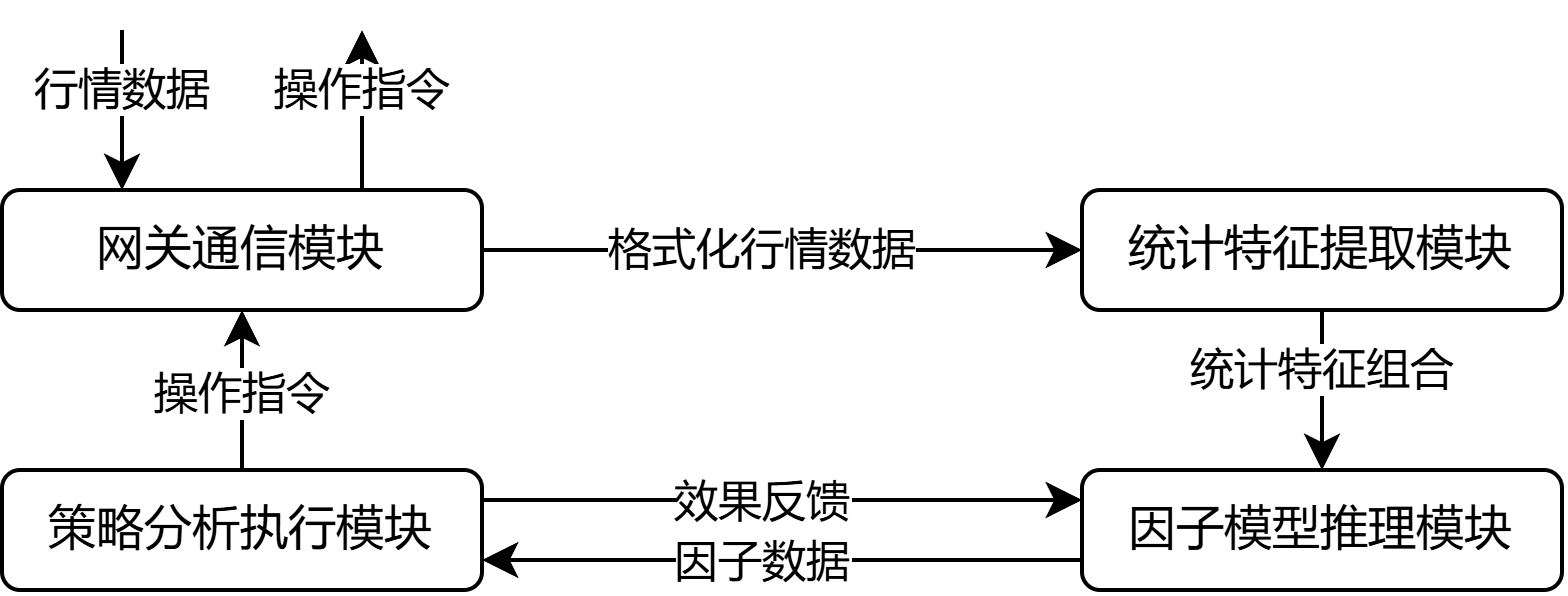
\includegraphics[width=1\textwidth]{image/chap02/lowlat.png}
    \caption{低延时交易系统基本架构}
    \label{fig:lowlatencysystem}
\end{figure}
低延时交易系统是量化交易的基础设施,其主要功能是在低延时的前提下完成市场行情的接收、分析与交易策略的执行。
如图\ref{fig:lowlatencysystem}所示,低延时交易系统以流水线的形式设计功能模块:
首先是网关模块,其负责接收和解析交易所的行情数据包,迅速将行情数据格式化后提交后续模块,确保数据实时与准确;
随后是数据预处理模块,接收格式化行情数据后更新内存数据库,然后对其进行清洗、标准化等操作,提取行情数据中的统计特征,为后续进一步分析提供基础;
接着是因子模型推理模块,该模块将预处理后的统计特征输入因子模型,然后执行计算推理,其输出作为对行情的表征;
最后是策略执行模块,依据因子模型的输出结果,决策和执行交易策略,向网关发送下单、撤单等操作请求,确保交易高效执行,同时向因子模型推理模块反馈信息。

为了实现高频交易下低延时的需求,低延时交易系统的设计与实现面临着诸多技术挑战。
整个交易流程关键路径的执行时间必须被严格控制在数十微秒之内,这对系统的每个模块都提出了极高的性能要求。
为此,交易系统中的各个模块均需要综合系统与硬件特性,从而尽可能提高系统执行效率,降低延时:
网关模块通过采用用户态网络库如DPDK甚至FPGA硬件加速技术,实现快速接收和解析行情数据;
数据预处理模块通过运用多线程并行处理与内存数据库如Redis以提高响应速度,或将模块编入内核态中完成数据清洗与标准化;
因子模型推理模块通过结合硬件架构调优算子,优化计算图与针对性的高效算法,显著降低模型推理延时;
策略执行模块则依赖高性能编程语言如C++和快速订单管理系统及直接市场接入(DMA)技术,以确保交易策略的高效执行。
在这一过程中,因子模型的推理计算尤其重要,由于其计算复杂度高,因此其推理延时在全过程延时中占有较大比例。
由此可见,提高因子模型的推理效率,降低其推理延时,就成为确保交易策略能够正确及时执行的关键所在。
这需要深入结合因子模型的结构特征,也需要对推理框架的架构设计和软件算法进行针对性的调整改进,以实现整个系统的高效运作。

\section{因子模型}

在低延时交易系统的运行过程中,因子模型推理模块通过将统计特征输入因子模型执行推理计算,从而向策略执行模块输出行情预测。
而因子模型作为量化交易行情表征的核心,设计的目标在于为行情建立模型,从中获取可用于策略分析的简易有效特征。
设计因子模型时,需从行情数据中挖掘出具有表征能力的特征因子,这些因子可以是行情基本面指标(如市盈率、市净率等),也可以是交易技术指标(如移动平均线、相对强弱指标等),也可以是宏观经济指标(如利率、通货膨胀率等)。
因子模型设计的最终目的在于通过统计和数学方法,建立因子与资产风险和收益间的定量关系,并借此探索因子影响资产未来收益的途径。


以公式\ref{con:inventoryflow}表示的动量因子为例,$\alpha_{i,t}$ 表示第 $i$ 个资产在时间 $t$ 的alpha因子值,$P_{t}$ 表示时间 $t$ 的资产价格,$P_{t-N}$ 表示时间 $t-N$ 的资产价格,$N$ 表示过去的时间窗口长度。
\begin{align}
    \begin{split}
        \alpha_{i,t} &= \frac{P_{t} - P_{t-N}}{P_{t-N}}, \\
    \label{con:inventoryflow}
    \end{split}
\end{align}
此类早期因子模型主要基于经验公式,直接对行情数据的某些统计量进行数学运算,一定程度上指示交易方向,但其表征市场行情特征的能力极其有限,难以应对复杂的市场环境。
尤其是伴随经验公式中超参数的引入,其调整难度和复杂性快速增加,实际应用价值逐步下降。
随着机器学习技术的发展,因子模型逐渐使用机器学习方法提高抗噪能力和表征水平。
现代因子模型,尤其是多分支因子模型,通过多分支结构综合处理多种行情指标,能够有效捕捉市场行情的复杂特征,极大提升了模型的表征能力和抗噪性能,为交易者提供了更为精准、可靠的决策依据,从而在激烈的市场竞争中占据优势。

多分支因子模型的输入通常是多种行情特征的拼接,在输入后切片进入不同的分支进行初步处理,随后通过计算操作融合各条分支,从而使得模型可以综合不同行情特征,并最终给出因子输出指示策略执行。
从输入模式方面,多分支因子模型的输入具有高度的可拓展性,其输入既包含了多个统计特征,但是又相互独立。
这使得多分支因子模型在计算过程相互独立的分支之间可以针对各分支输入实现优化算法。
在结构特征方面,多分支因子模型其整体结构类似树状收敛,分支之间融合后形成唯一的新分支,最终汇集为模型的唯一输出。
这种结构综合分析了多个分支的特征,有效提高了模型的性能,尤其是残差连接\cite{he2015deepresiduallearningimage}大幅提高了模型设计的可用深度,多分支因子模型因此具有更强的综合能力。
\begin{figure}[h]
    \centering
    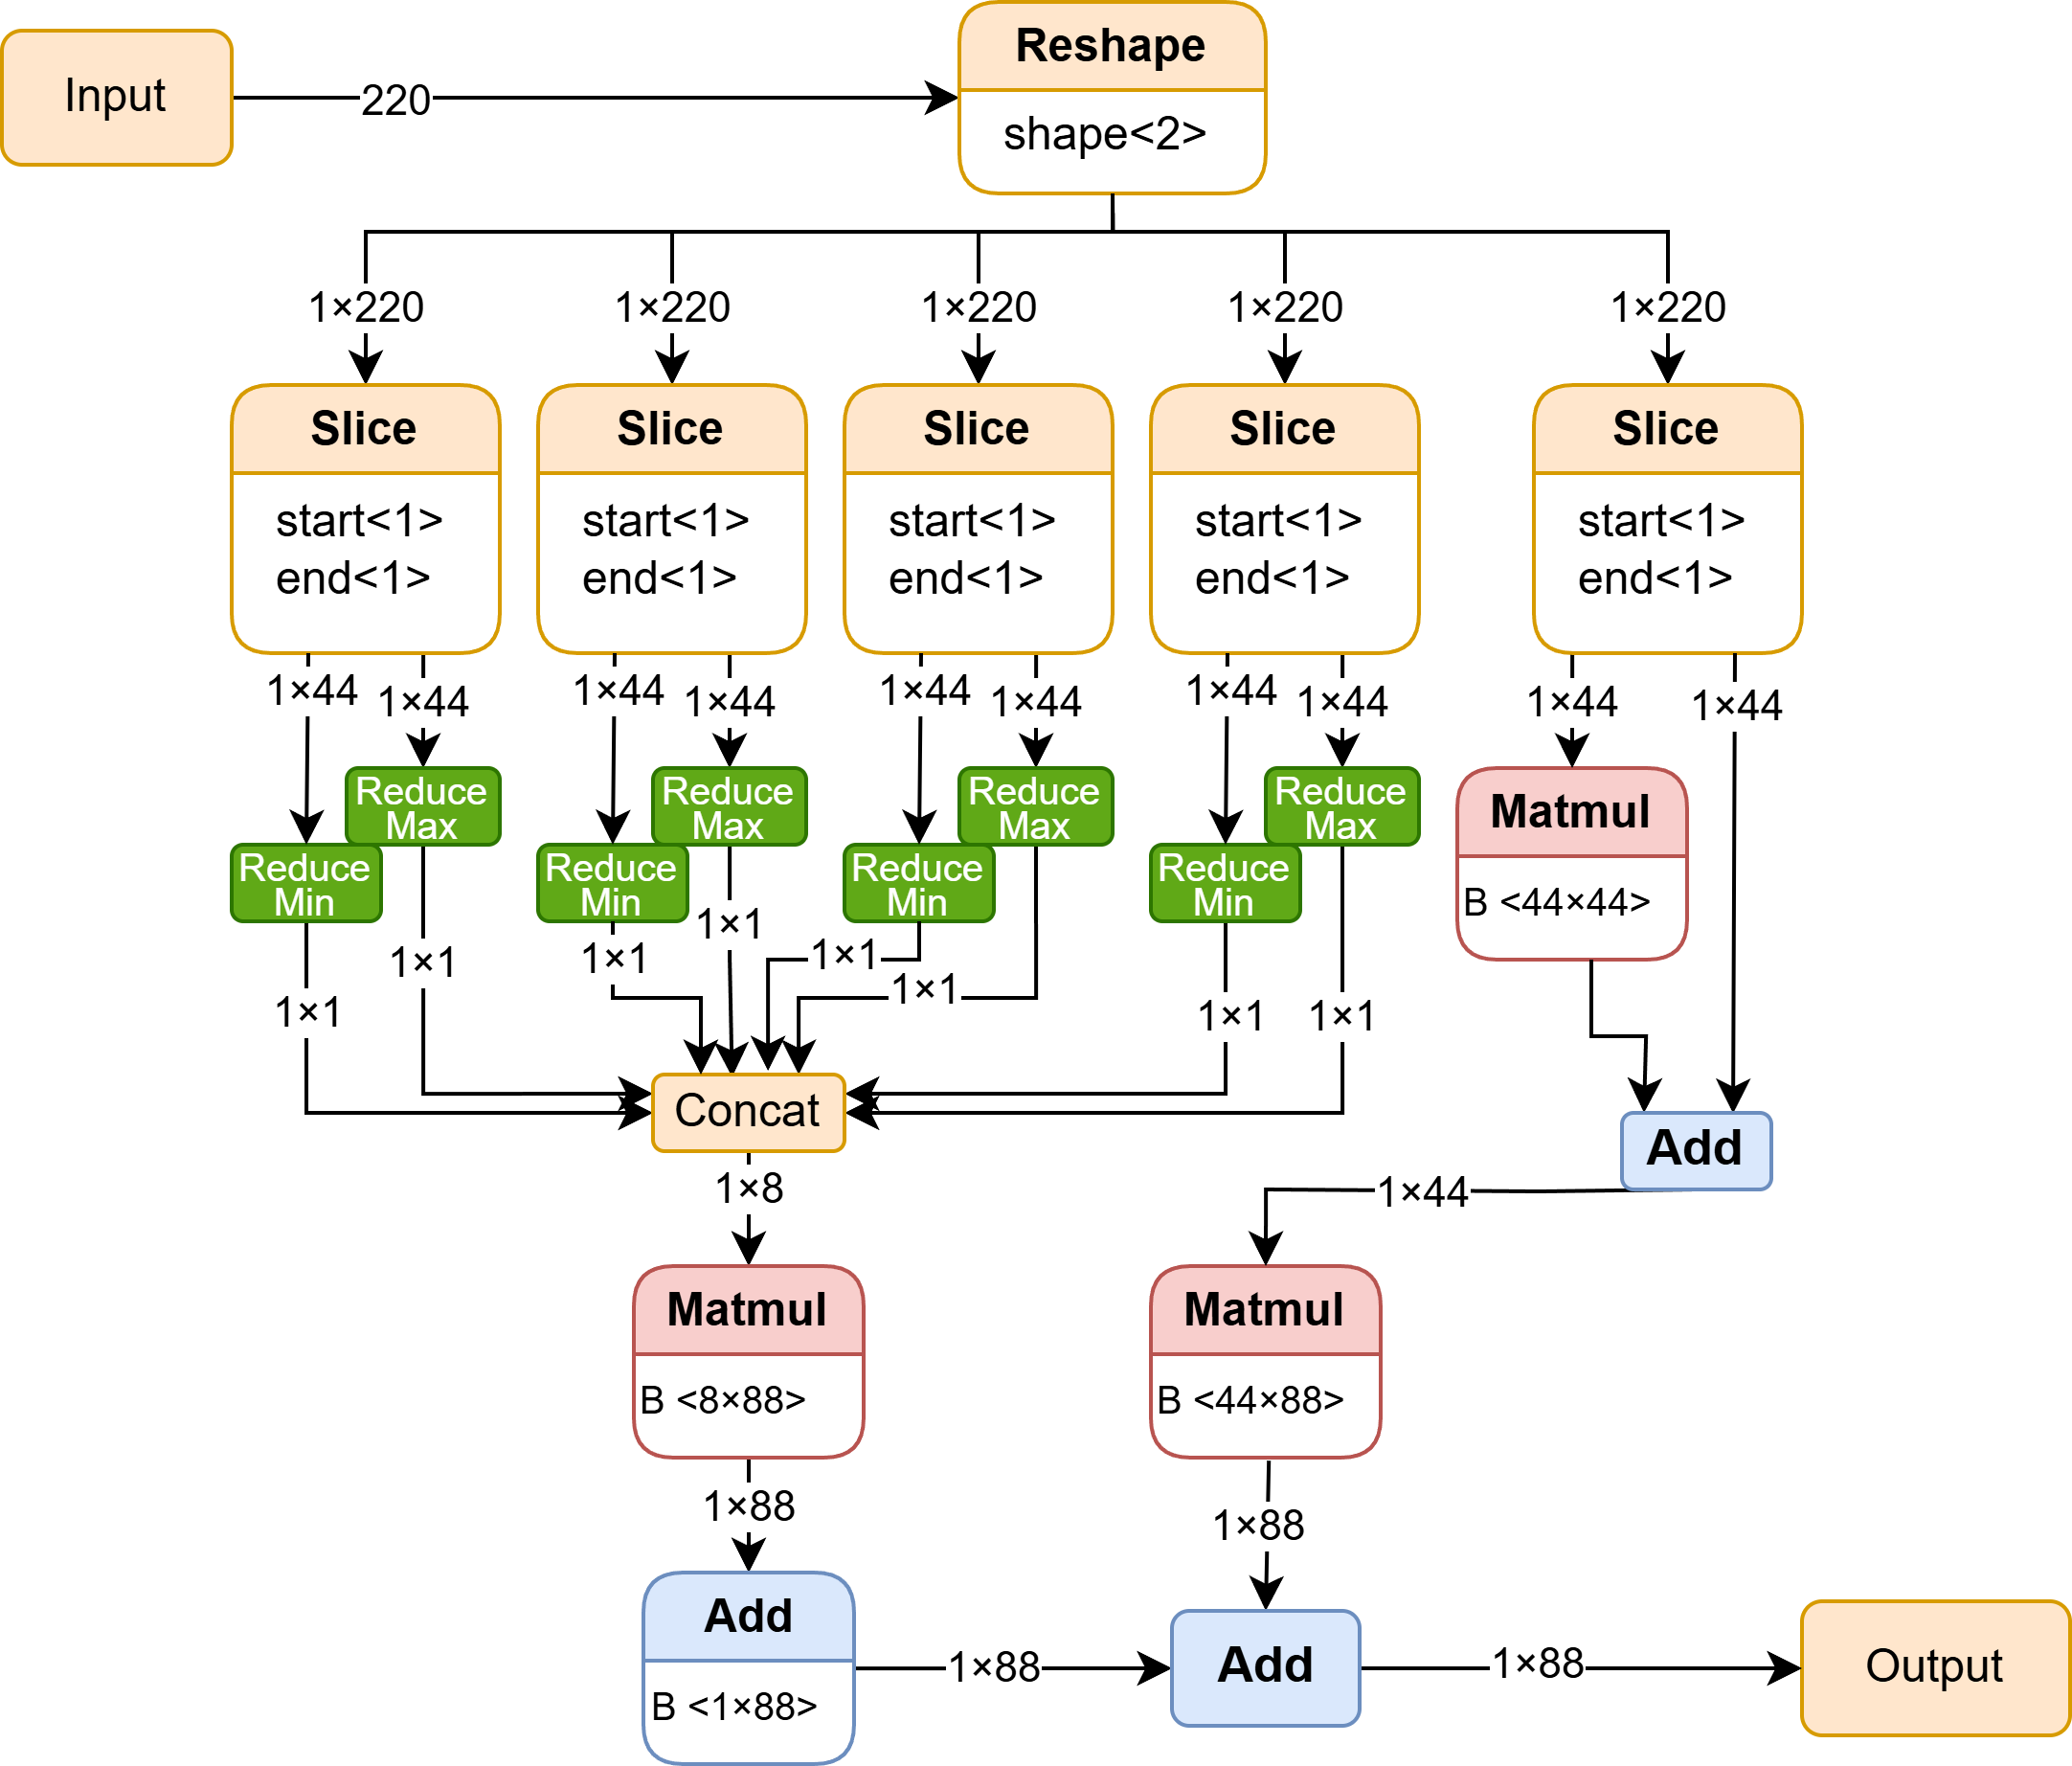
\includegraphics[width=1\textwidth]{image/chap02/models1.png}
    \caption{多分支因子模型样例}
    \label{fig:models}
\end{figure}


\section{模型推理框架}

在服务端高并发业务场景下,现有的多数推理框架侧重于处理大量请求的并行计算,通过分布式架构和异构计算来提高系统的吞吐量。
然而,低延时交易系统所面临的场景则截然不同,其优化的目标在于实现单样本高频率计算密集场景下的极低延时。
这就要求推理框架能够充分利用因子模型的结构特征与输入模式,通过针对性的优化策略,如内存映射、模型剪枝、算子融合等技术,有效提高模型整体的计算效率,降低推理延时。

当前多数模型推理框架仅针对服务端高并发场景进行了优化,对于高频交易的低延时要求缺乏针对性的解决方案。
然而即便优化的目的指标不同,现有推理框架的架构设计和技术应用对于低延时系统中的推理框架设计仍然具有参考意义。
例如,Tencent TFCC通过使用MLIR(多级中间表示)技术实现了自动算子融合,极大减小了由于算子编码调优而浪费的时间和人力,并显著降低了推理延时,
同时基于MLIR的优化路径机制具有极强的可拓展性,优化路径之间彼此解耦合,具有极高的优化上限。
llama.cpp则作为一个高度优化的C/C++实现,专注于本地LLM推理性能的优化,充分利用了现代CPU架构中的SIMD指令集,为多个LLM工具和应用提供了基础运行时支持,
其使用Protobuf作为模型的解析器,通过C++将模型进行进一步的包装和抽象,拓展了模型结构,同时为进一步优化提供开发空间。
TensorRT是NVIDIA推出的一个高性能深度学习推理优化模块和运行时引擎,其包括静态计算图优化和动态推理优化两个解耦合的基本过程,
其静态计算图优化过程向上对模型适配,而动态推理优化过程向下对硬件适配,取得了优异的性能。

除了现有模型推理框架的架构设计和技术应用外,因子模型的推理框架还应当面向系统和硬件做出针对性优化。
例如,在推理的执行过程中,缺页中断将导致严重的延时增长,因此使用大页的内存映射和内存锁定方法,能够在系统运行全过程内不发生缺页中断,有效提高访存性能。
利用系统调度指定CPU核心隔离操作,可以尽可能减少无关进程在指定核心的运行,从而有效提高CPU的占用时间。
在这些推理框架中,面向硬件的优化也是一个关键环节。
在日志系统的计时过程中,使用rdtscp指令计数器参与计时,能够以多核一致性clock的细粒度进行计时,完成高精度的性能测试。
通过针对特定硬件架构的算子实现,可以充分利用硬件的并行计算能力,提高计算效率。

总体来看,在模型推理框架的整体设计上,应当效仿先进的架构设计和技术应用,这将有效提高优化手段的效果上限。
同时在具体的内存管理和系统配置等方面,也要充分利用相关系统属性进行优化以提高访存和计算效率。
只有在综合多种优化手段的前提下,模型推理框架才能够在高频交易的低延时环境下有优越的性能表现。

\section{高频交易下CPU计算架构}

尽管当前模型推理的硬件设备以GPU为主,但以业内普遍使用的英伟达A100计算卡为例,从CPU发起空核函数到GPU执行核函数之间的延时就高达2.59微秒,而连续空核函数之间的间隔延时约为5微秒。
而在更早的特斯拉架构中,发起矩阵乘操作核函数,其间隔延时高达20微秒,使其不具有应用价值。
\begin{figure}[h]
    \centering
    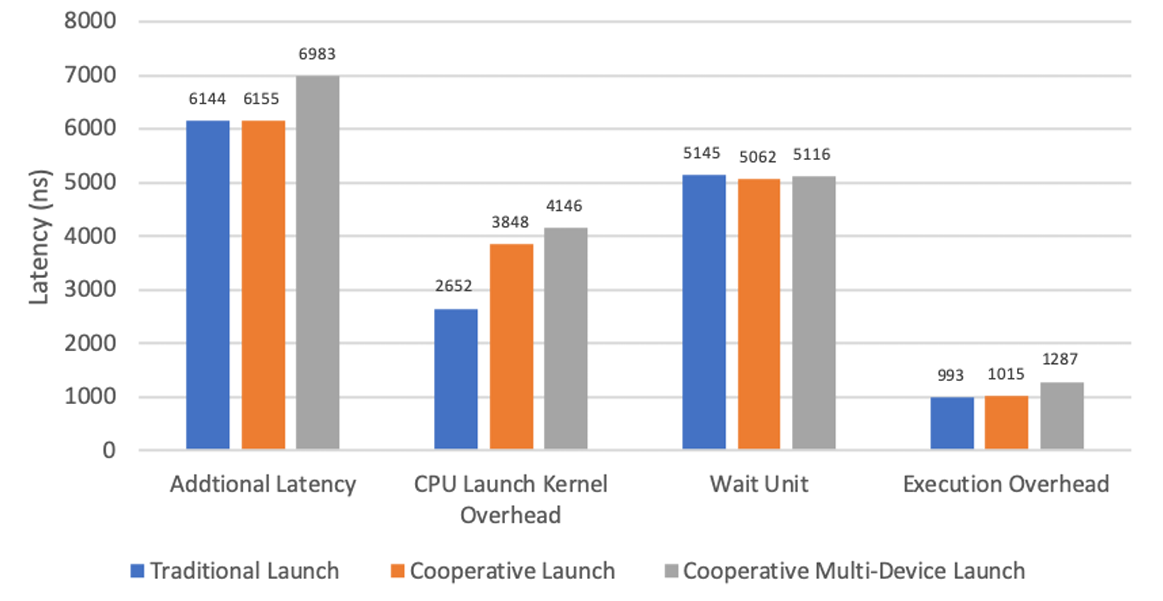
\includegraphics[width=1\textwidth]{image/chap02/Overhead.png}
    \caption{使用不同方法发射大型核函数的执行延时组成}
    \label{fig:kernelss}
\end{figure}
如图\ref{fig:kernelss}所示,图中Traditional Launch,就是CUDA程序中常用语法糖发射的接口;
Additional Latency代表额外的延迟,是CPU刚刚调用了一个发射核函数后发射另一个核函数的额外延迟;
CPU Launch Kernel Overhead代表CPU调用发射函数到GPU执行的延迟;
Wait Util是核函数的内容,测试过程中通过多次调用Wait定时函数来填充核函数;
Execution Overhead指GPU的实际执行时间和Wait定时函数执行时间的差值。
可以观察到,在加入参数和数据传输后,延时已经使得因子模型在以期货市场为核心的高频交易中失去竞争力。
此外,尽管在多数工程计算场景如有限元计算中,计算过程通常被整体编码为一个核函数,
但对于时刻变化的业务模型,包括交易因子模型在内,为了维持项目的可读性和可维护性,不可避免地对计算节点进行抽象,进而将整个模型抽象为一个由算子组成的计算图。
在这种抽象计算图的推理过程中,算子核函数的连续发起导致仅累计启动延时就已超出预期。
因此,因子模型推理的目标硬件普遍使用服务器高性能多核CPU,尤其以AMD EPYC和Intel Xeon为业务主流硬件。


\begin{figure}[h]
    \centering
    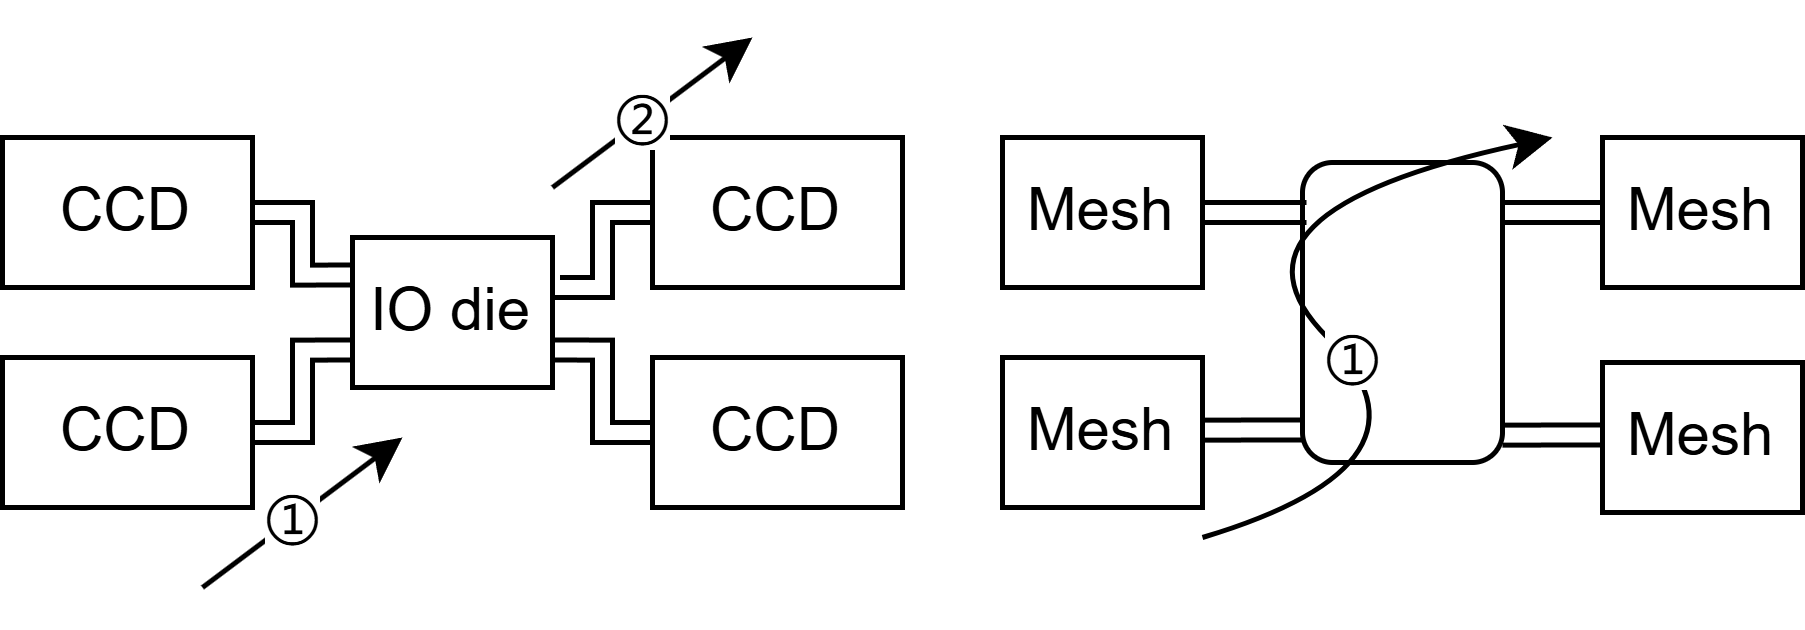
\includegraphics[width=1\textwidth]{image/chap02/arch.png}
    \caption{AMD EPYC与Intel Xeon在CPU NUMA访存过程对比}
    \label{fig:cpus}
\end{figure}

在高频交易场景下,CPU的架构特性对因子模型的实际推理模式和效率有显著的影响,为此,优化方案需要围绕如何提高CPU利用率来设计开发。
现在主流的CPU架构里,AMD EPYC和Intel Xeon在多核的拓扑封装方面存在着显著的差异,如图\ref{fig:cpus}所示:
AMD EPYC架构基于CCX和CCD的核簇模式设计,在单个核簇内多个核心共享L3缓存,借助核簇内的高速通信总线和大L3缓存,相比较Intel Xeon在多线程、大规模数据的计算场景下具有显著的性能优势。
Intel Xeon在拓扑封装方面则采用环路架构,核心间通过环形总线通信,相比AMD EPYC,通信延时明显下降,其在单线程性能和跨核访存方面具有优势,
能快速处理高频率单样本的计算任务,更符合低延时交易系统需求。同样在高频交易中常用的一读多写场景中,其广播延时和多播延时比AMD EPYC有明显的改善。
如图\ref{fig:cpus}所示,AMD EPYC处理器在跨核心访存过程中相比较Intel Xeon处理器存在路由的中间过程,而在多个业务实例部署且跨核通信密集的场景下,IO die的路由效率极其有限,这直接导致AMD EPYC相较于Intel Xeon有更高的一致性延时。
除了拓扑封装的差异导致跨核通信的性能差异外,两者在指令集支持上也有诸多不同,这也决定了它们在不同计算场景下的适用性。
Intel Xeon在支持AVX512指令集方面表现出色,而AMD EPYC在连续数个版本只使用AVX2模拟AVX512来实现指令集兼容。
因此,对于某些SIMD高需求的应用如向量数据库,AMD EPYC的计算性能就略显不足。
综上所述,框架实际的优化方案必须结合具体业务场景和CPU架构特性以设计实现,如此才能达到最优性能。
充分利用不同CPU架构的特性,是改善推理过程延时的关键。

为了把CPU的计算能力发挥到极致,目前已有多种高性能计算库针对不同CPU架构实现针对性性能优化。
以Intel MKL和AMD AOCL为例,其分别为Intel Xeon和AMD EPYC处理器提供高效的计算操作接口。
通过调用常用的BLAS操作接口,开发者能够迅速实现对目标应用的性能调优。
Intel MKL GEMM JIT是Intel MKL推出的专注于小规模矩阵乘的高效计算接口,
通过即时编译技术生成针对特定矩阵尺寸和数据类型的高效计算代码,从而提升矩阵运算性能。
Blaze HPC是个高效的数值计算库,在算子调优的流水线中,通常作为最后一级编译输出的部分,通过将已完成设备指令集适配的BLAS传入Blaze HPC,
然后向其配置文件写入CPU的指令集和各级缓存信息,算子即可实现细粒度的自动调优以实现最优性能。
它通过高度优化的算法和数据结构,有效提高CPU计算的利用率,加速数值计算过程。
Blaze HPC还支持张量运算,为因子模型推理框架提供了基本的高性能算子实现,让CPU在高频交易场景下能高效完成复杂计算任务。